\documentclass[12pt]{article}
\usepackage[utf8]{inputenc}
\usepackage{graphicx}
\usepackage{subcaption}
\usepackage{amsmath} 
\usepackage{fancyhdr} 
\usepackage{geometry} 
\usepackage{dirtytalk} 
\usepackage[english]{babel}
\usepackage{csquotes}
\usepackage{hyperref}
\usepackage{listings}
\lstset{
    language=C,
    basicstyle=\ttfamily, 
    numberstyle=\tiny,
    frame=single,
    breaklines=true,
}

\begin{document}
\begin{titlepage}
\begin{center}
    
\includegraphics[width=0.3\textwidth]{image.png} \\[0.2cm]
    
    \textbf{MINISTRY OF EDUCATION, CULTURE AND RESEARCH 
OF THE REPUBLIC OF MOLDOVA} \\[0.3cm]
    
    \textbf{Technical University of Moldova 
Faculty of Computers, Informatics and Microelectronics 
Department of Software and Automation Engineering} \\[2cm]
    
    \textbf{Postoronca Dumitru FAF-233}\\[0.5cm]
    
    \Huge \textbf{Report} \\[0.5cm]
    
    \large Laboratory Work №4\\[0.5cm]
    
    \textbf{of AA} \\[3cm]
    
    \begin{flushright}
        \textit{Checked by:} \\
        \textbf{Fistic Cristofor}, \textit{university assistant} \\
        DISA, FCIM, UTM
    \end{flushright}
    
    \vfill
    
    Chișinău -- 2024
\end{center}
\end{titlepage}

\newpage
\setcounter{page}{1}
\pagestyle{fancy}
\fancyhf{}
\rhead{\thepage}
\lhead{FAF-233 Postoronca Dumitru ; Laboratory work №4}

\section*{Conditions of the Task}
Dynamic programming is defined as a computer programming technique 
where an algorithmic problem is first broken down into sub-problems, 
the results are saved, and then the sub-problems are optimized 
to find the overall solution — which usually has to do with finding 
the minimum distance in the shortest path problem.
\begin{enumerate}
    \item Implement in a programming language the algorithms of Dijkstra and Floyd–Warshall using dynamic programming.
    \item Perform empirical analysis of these algorithms on both sparse and dense graphs.
    \item Increase the number of nodes in graphs and analyze how this influences algorithm performance.
    \item Make a graphical presentation of the data obtained.
    \item Draw conclusions based on the analysis performed.
\end{enumerate}

\clearpage
\section*{Input data}
\hspace{0.8cm}
To analyze and compare the pathfinding algorithms, we define the following input data conditions:
\begin{enumerate}
    \item Number of edges
      \begin{itemize}
        \item Sparse graph 
        \item Dense graph 
      \end{itemize}

    \item Edge Cases:
      \begin{itemize}
        \item Negative weights (Floyd–Warshall supports them; Dijkstra does not)
        \item Cyclic graphs
      \end{itemize}
\end{enumerate}

Input data was generated by a special function written in JS that takes as input 
the wideness of the graph (number of direct children each node will have) and its depth.
Total number of nodes is calculated using the formula: $$N_{nodes} = width^{depth}$$

\clearpage
\section*{Metrics in Algorithm analysis}

In this laboratory work I test how each pathfinding algorithm performs 
depending on the number of edges

For this purpose I run the same algorithm
to find the shortest path from the root node to a leaf node at various depths.
If the depth of the generated graph is 5, I measure metrics for: depth 1 through depth 5.


\subsection*{Algorithms Implementation}


Implementation of the algorithm was done using python and visual representation 
is done using matplotlib.

\subsection*{Results}
After running the tests, the following results were obtained:

\begin{figure}[h]
    \centering
    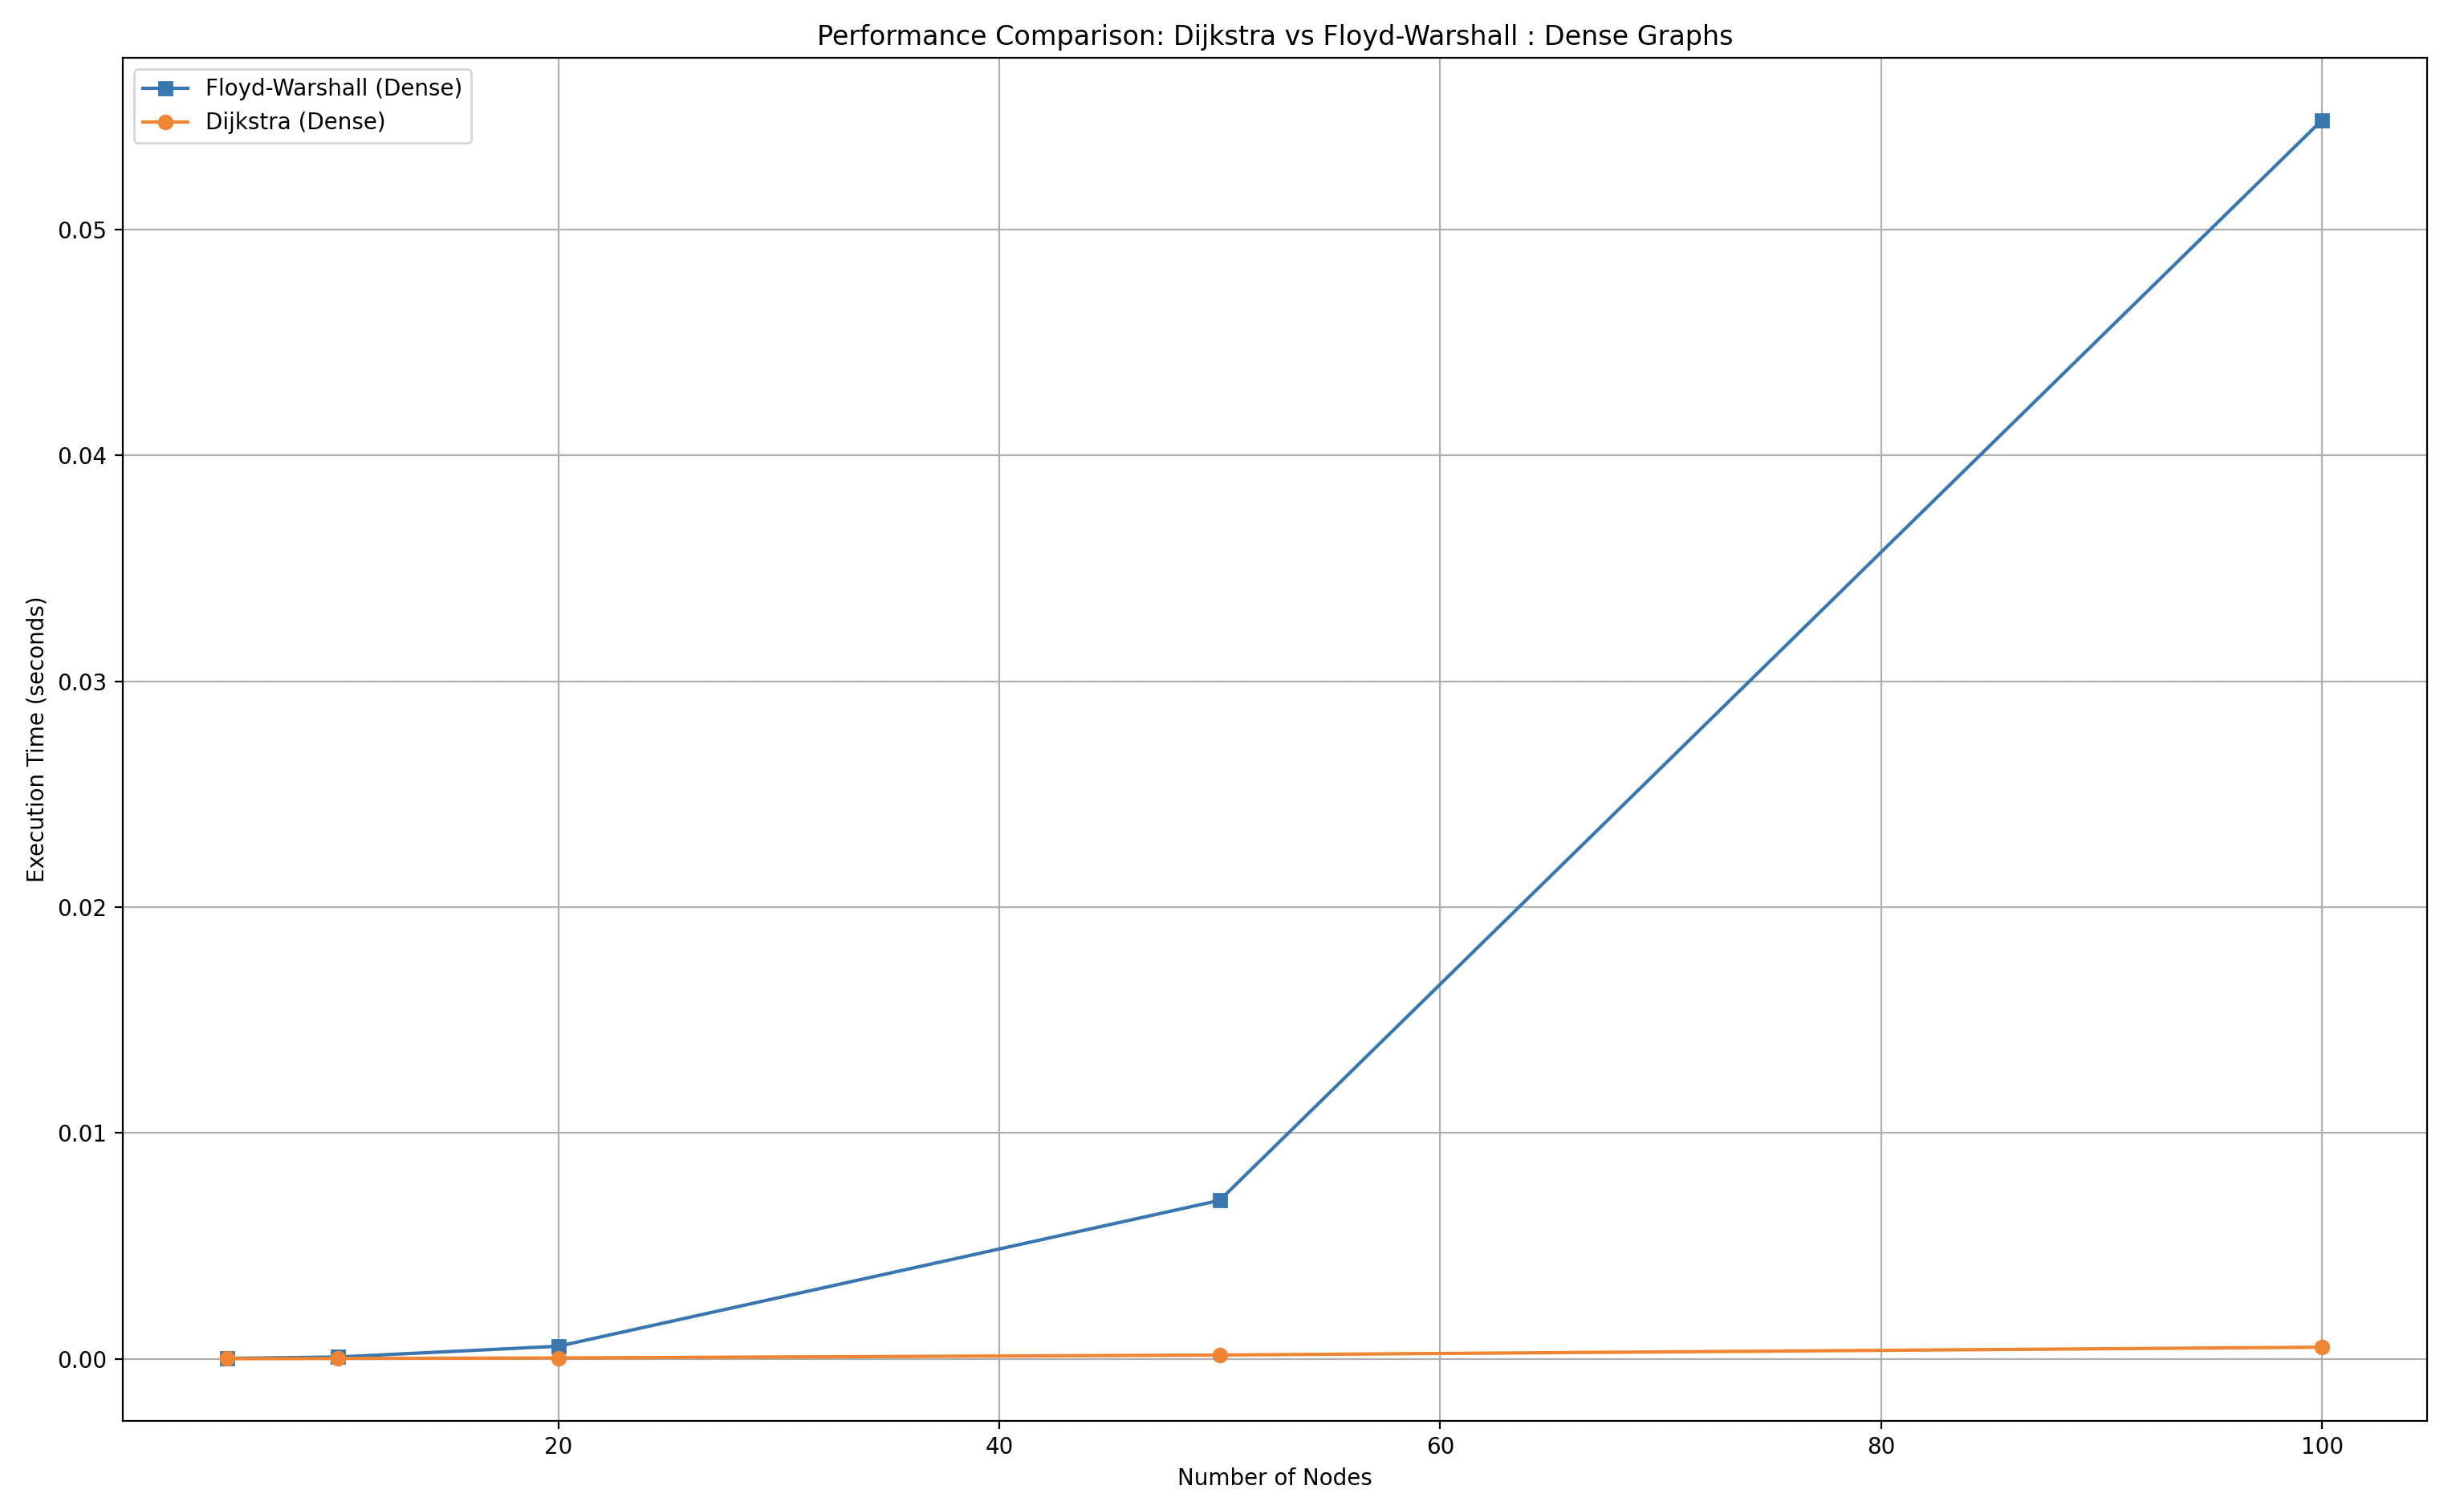
\includegraphics[width=1\textwidth]{images/dense.png}
    \caption{Pathfinding comparison for a dense graph}
    \label{fig:w20d4}
\end{figure}


\begin{figure}[h]
    \centering
    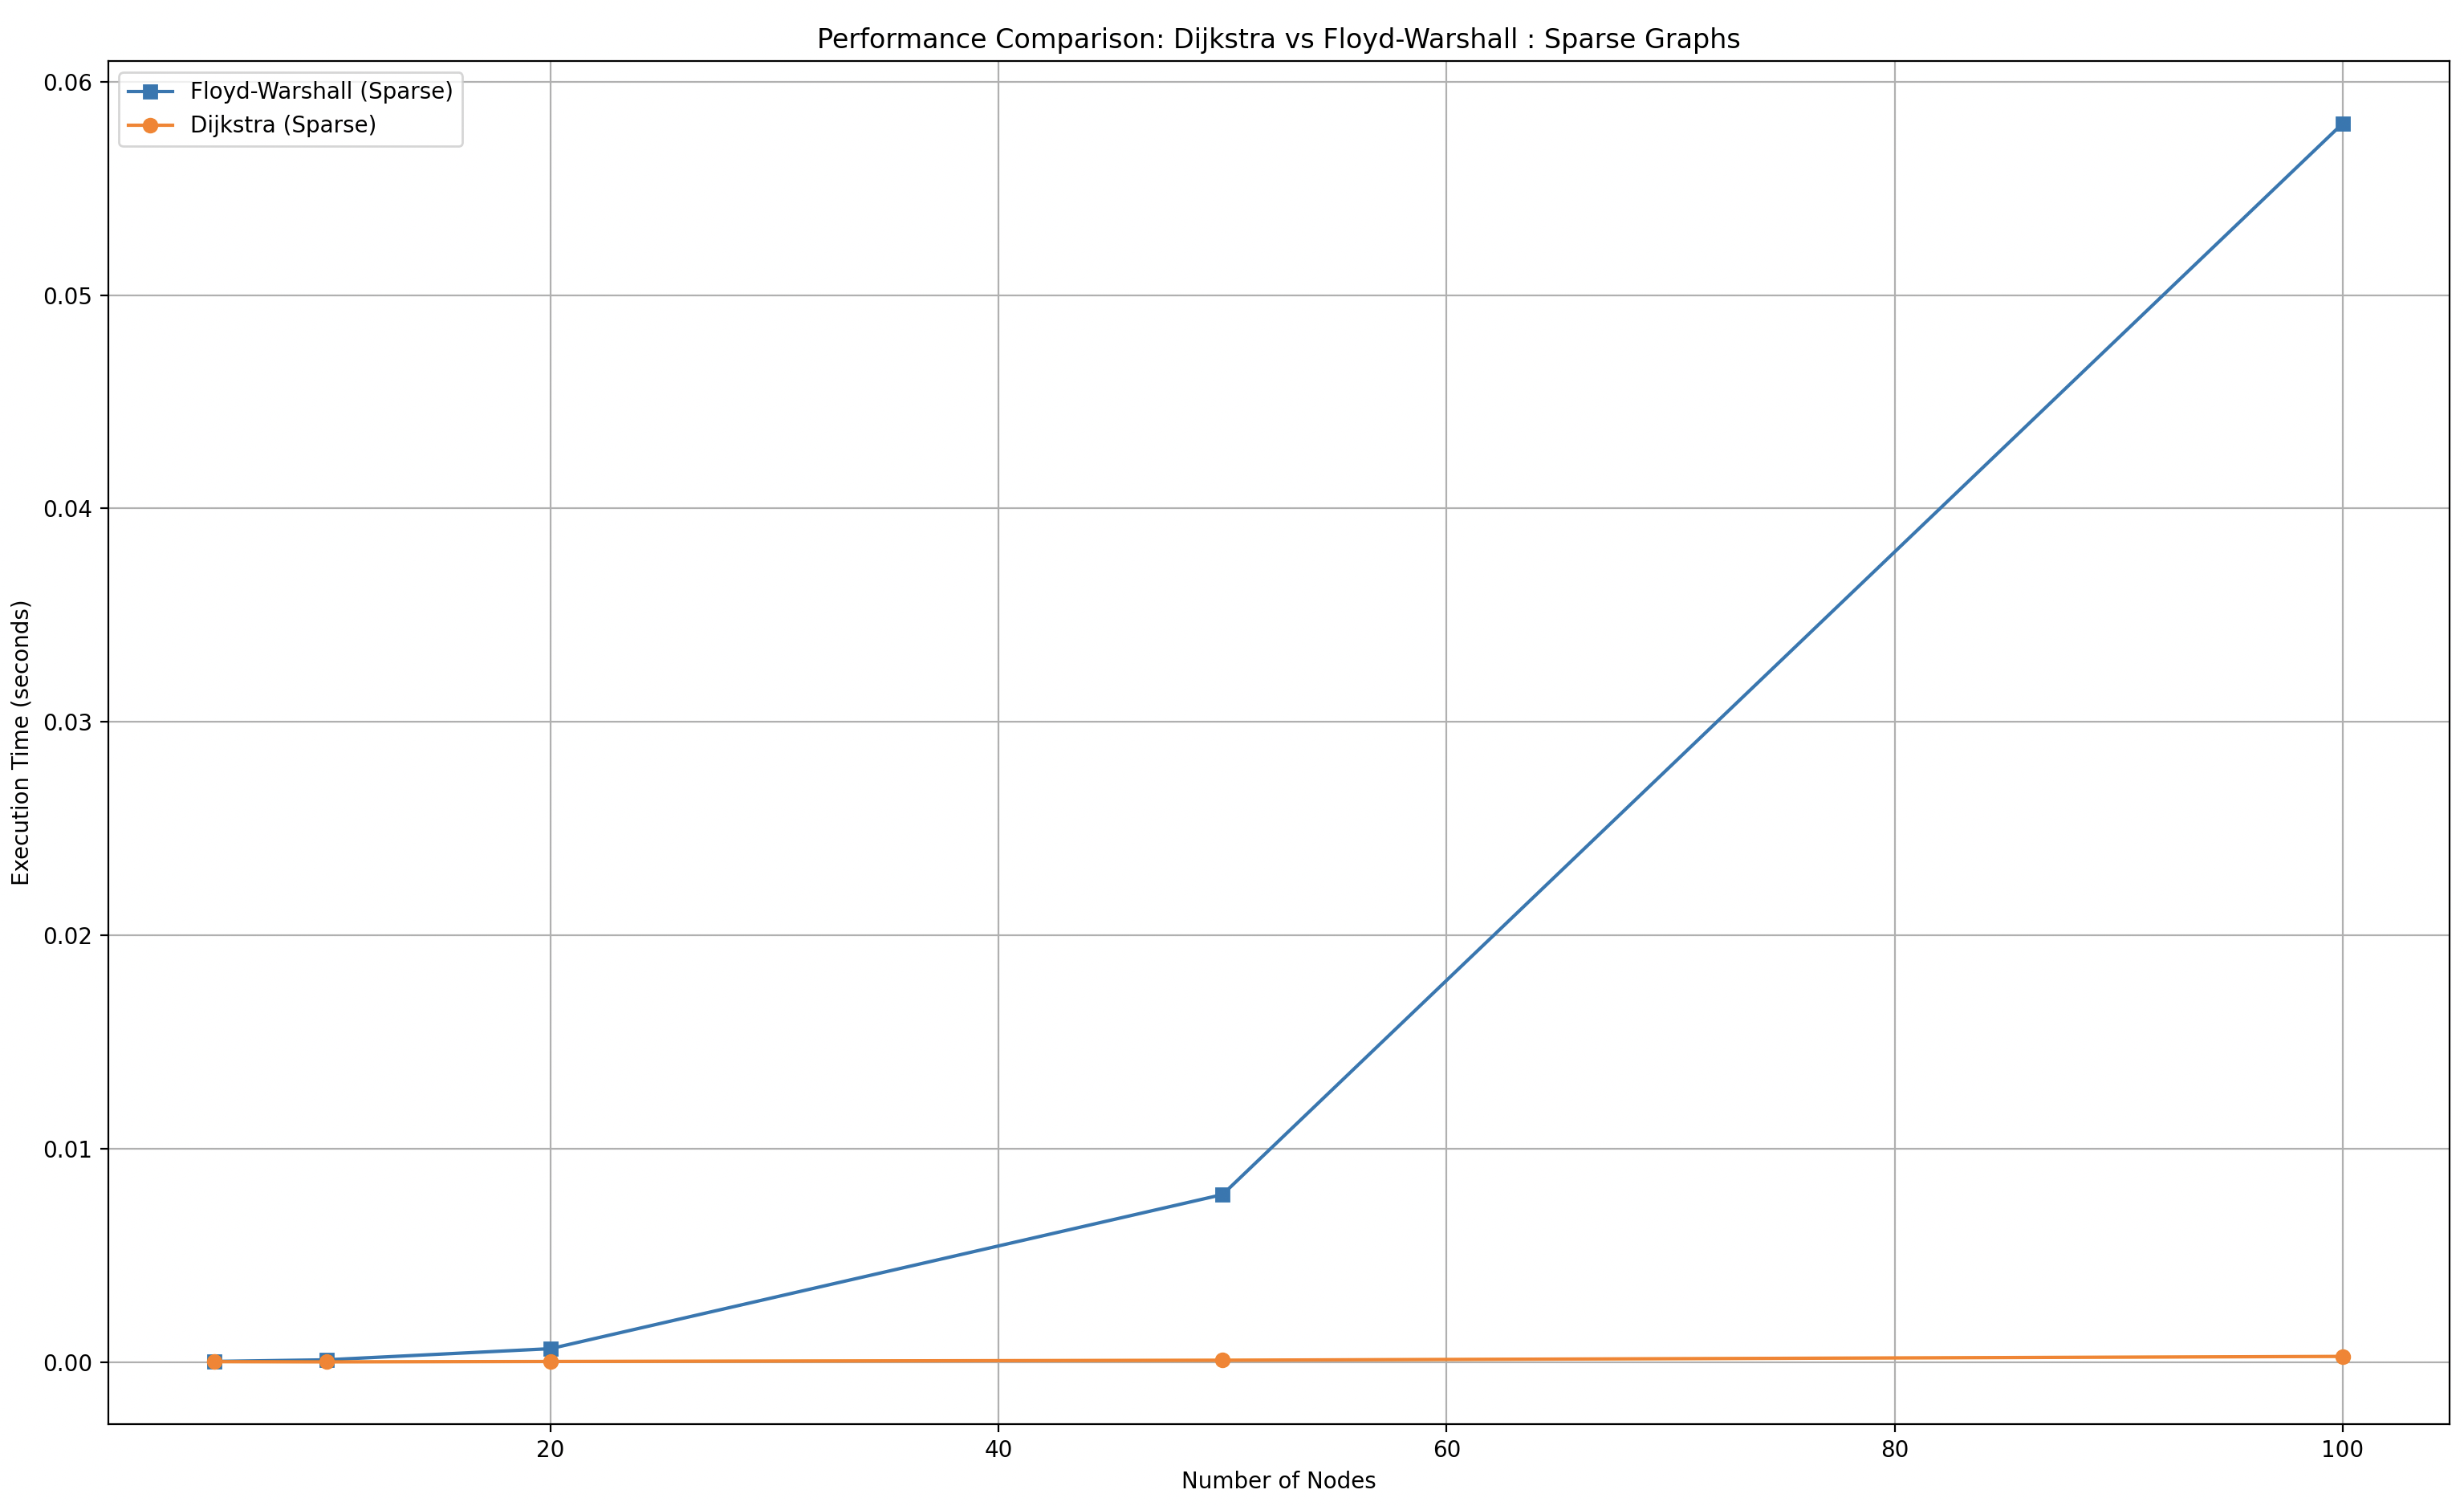
\includegraphics[width=1\textwidth]{images/sparse.png}
    \caption{Pathfinding comparison for a sparse graph}
    \label{fig:w3d11}
\end{figure}

\clearpage

As observed in the results, the Dijkstra algorithm performs efficiently for graphs without negative weights, 
providing accurate shortest paths and generally being faster on sparse graphs due to reduced edge exploration.

Floyd–Warshall, on the other hand, calculates all-pairs shortest paths and is more suited for dense graphs.
It gracefully handles negative weights but has higher time complexity.

The time complexities are:

\begin{itemize}
  \item \textbf{Dijkstra:} \(O((V + E)\log V)\) with a priority queue
  \item \textbf{Floyd–Warshall:} \(O(V^3)\)
\end{itemize}

Despite its simplicity and power, Floyd–Warshall becomes impractical for large graphs due to its cubic time complexity.

\section*{Graphical Representation}
\hspace{0.8cm}
A web-based visualization was developed to demonstrate how Dijkstra and Floyd–Warshall algorithms operate.
It can be accessed online\cite{site}.

The user interface provides the following features:
\begin{itemize}
  \item Recieve different combinations of the edges and weights at each reload
  \item Switch between Dijkstra and Floyd–Warshall
  \item View execution logs for analysis
\end{itemize}

\begin{figure}[h]
    \centering
    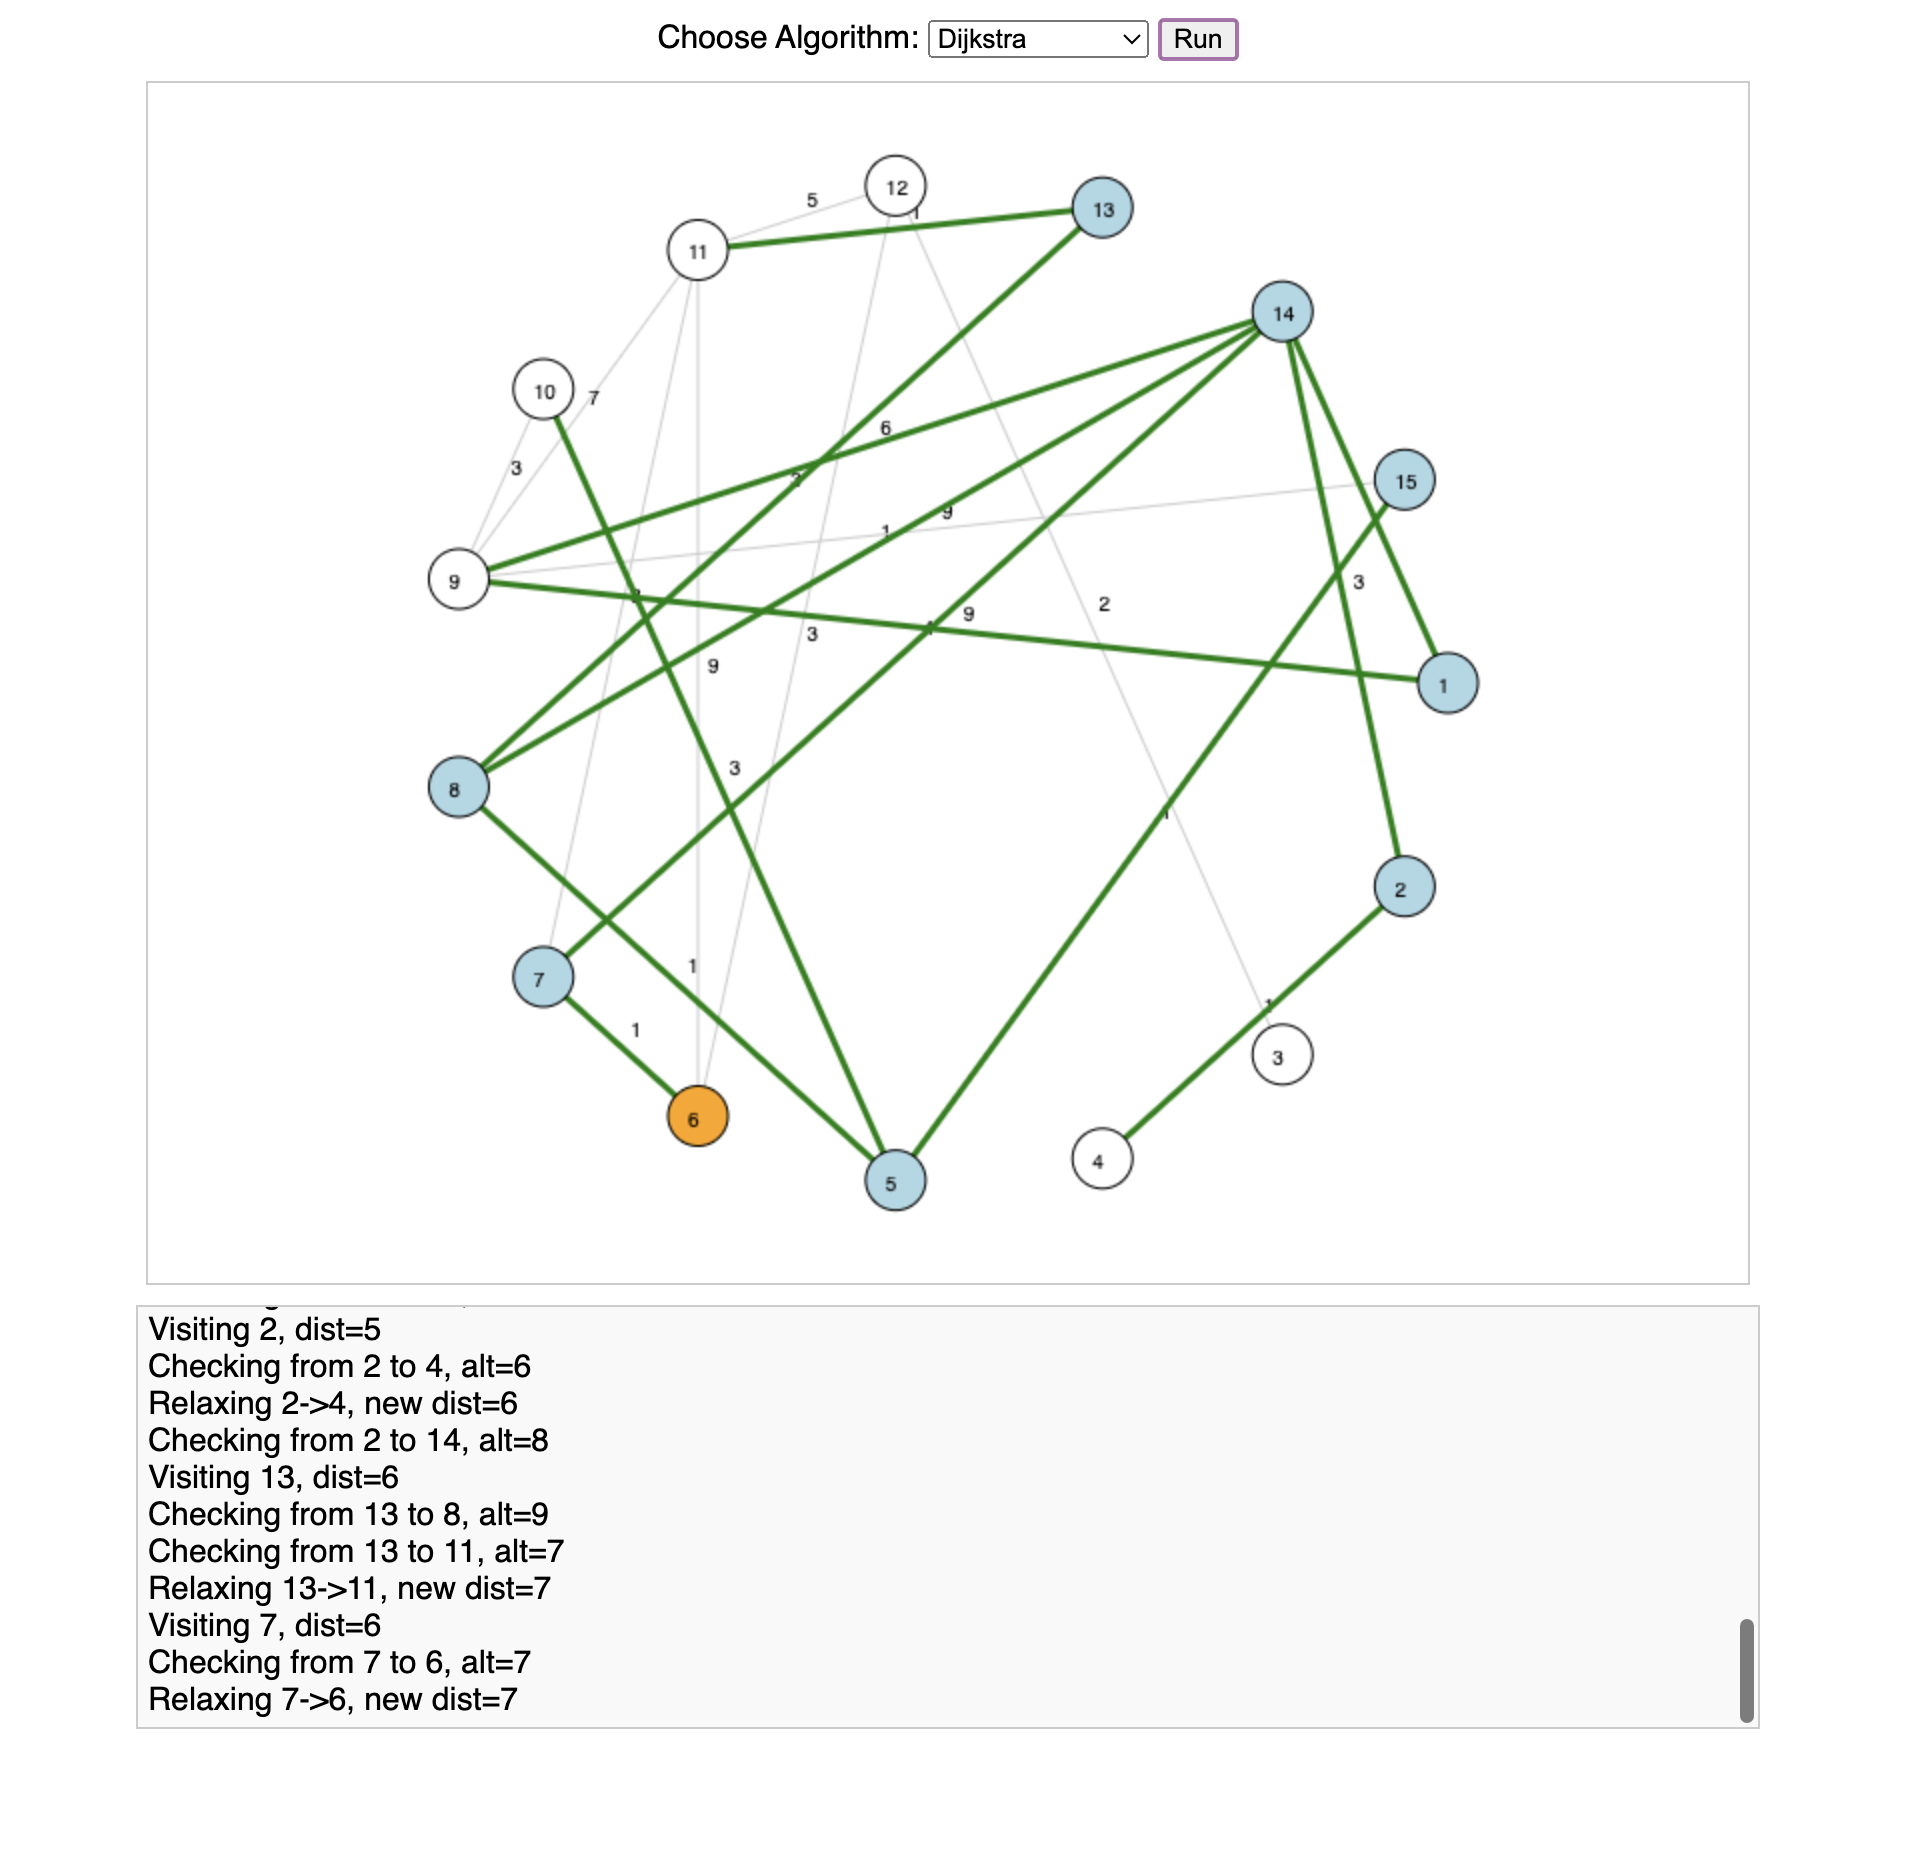
\includegraphics[width=1\textwidth]{images/site_dijkstra.png}
    \caption{Graphical representation of Dijkstra and Floyd–Warshall algorithms}
    \label{fig:site}
\end{figure}

\begin{figure}[h]
    \centering
    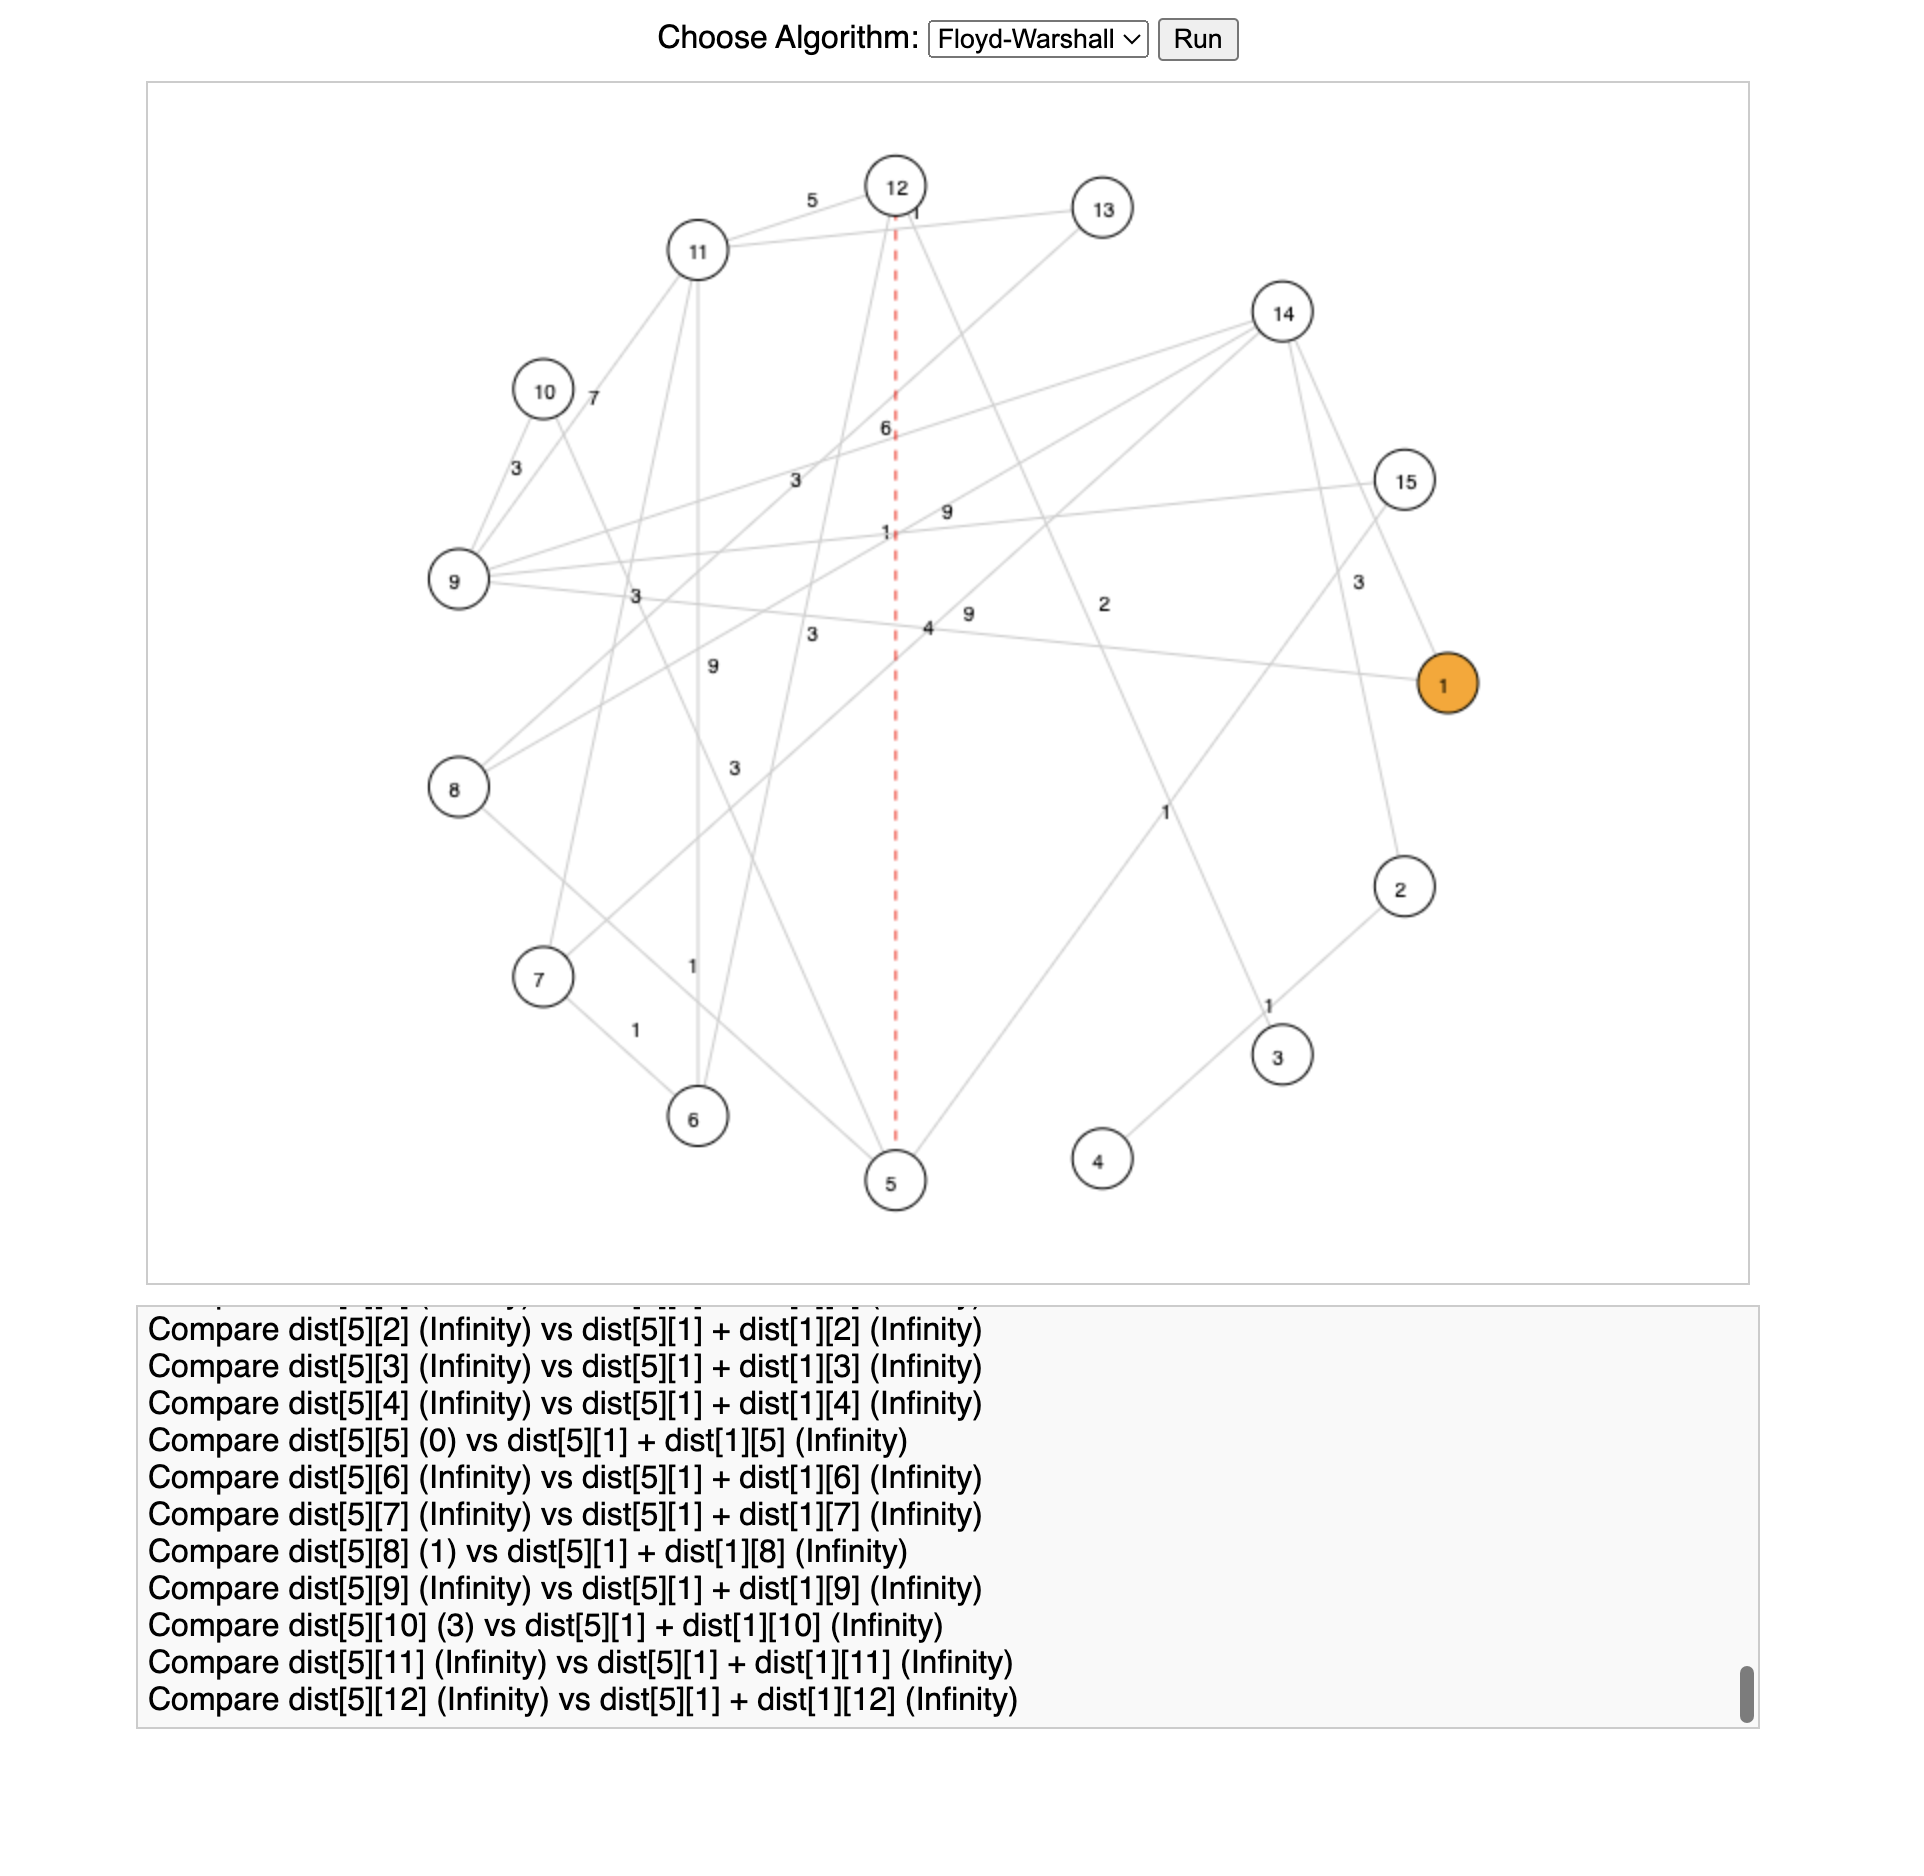
\includegraphics[width=1\textwidth]{images/site_warshall.png}
    \caption{Graphical representation of Dijkstra and Floyd–Warshall algorithms}
    \label{fig:sitewarshall}
\end{figure}

\section*{Conclusion}

In conclusion I can say that Dijkstra is a very powerful path finding algorithm due to its low
time complexity and performs efficiently in finding the shortest path between 2 points.

But Floyd-Warshall algorithm is also a valid variant of finding the shortes path in cases when we need a 
full information about each of the nodes on a graph. Besides that Floyd-Warshall can handle negative weights
and graphs with negative cycles, which Dijkstra just cann't do.


\clearpage
\begin{thebibliography}{9}

  \bibitem{bytecoderef} \href{https://medium.com/dailyjs/understanding-v8s-bytecode-317d46c94775}{Franceska
      Hinkelman (2017) - Understanding bytecode \emph{Medium}}
  \bibitem{github} \href{https://github.com/DdimaPos/AA-labs/tree/main/Lab4}{GitHub repository of current laboratory work}
  \bibitem{site} \href{https://dfs-bfs-visualization.vercel.app/}{Graphical representation of Dijkstra and Floyd–Warshall}
\end{thebibliography}
\end{document}
